% !TEX encoding = UTF-8 Unicode
% !TEX spellcheck = en_US
%
\documentclass[runningheads]{llncs}
%
\usepackage{paralist}
\usepackage{graphicx}
\graphicspath{{../figures/}}
\usepackage[T1]{fontenc}
\usepackage[utf8]{inputenc}
\usepackage{color, colortbl}
\usepackage{bm}
\usepackage{amsmath}
%\newcommand{\ok}{{\color{green}\checkmark}}
%\newcommand{\no}{{\color{red}$\boldsymbol\times$}}
\newcommand{\ok}{{yes}}
\newcommand{\no}{{no}}
\newcommand{\transp}[0]{{\mathrm{T}}}
% Theorem environment for "Test x."
%\spnewtheorem{property}{Property}{\bfseries}{}
\spnewtheorem{test}{Test}{\itshape}{}

% If you use the hyperref package, please uncomment the following line
% to display URLs in blue roman font according to Springer's eBook style:
\usepackage{url}
\renewcommand\UrlFont{\color{blue}\rmfamily}
\usepackage[draft]{hyperref}

\begin{document}
%
\title{A Maple Toolchain for Rigid Body Dynamics of Serial, Hybrid and Parallel Robots}%\thanks{}}
%
\titlerunning{Maple Toolchain for Robot Rigid Body Dynamics}
% If the paper title is too long for the running head, you can set
% an abbreviated paper title here
%
\author{Moritz Schappler\orcidID{0000-0001-7952-7363} \and Tim-David Job \and Tobias Ortmaier}
%\author{Moritz Schappler\orcidID{0000-0001-7952-7363} \and Tim-David Job\orcidID{0000-0002-0609-3362} \and Tobias Ortmaier\orcidID{0000-0003-1644-3685}}
%
\authorrunning{M. Schappler et al.}
% First names are abbreviated in the running head.
% If there are more than two authors, 'et al.' is used.
%
\institute{
	Institute of Mechatronic Systems, Leibniz University Hannover, Germany\\
	\email{\{moritz.schappler,tim-david.job,tobias.ortmaier\}@imes.uni-hannover.de}}
%
\maketitle              % typeset the header of the contribution
%
\begin{abstract}
A new Maple toolchain for generating rigid body dynamics in symbolic form for robot manipulators is presented.
The peculiarity compared to existing tools lies in the framework of Bash scripts controlling the full workflow of the toolchain with a high degree of automation. 
The optimized Matlab code generated by Maple is automatically converted to function files with proper documentation and input assertions.
This renders manual post-processing of the results unnecessarily.
The focus of the paper is on the implemented unit-testing framework according to the method of test-driven development.
By providing the test framework together with the generated code in a stand-alone version, a good test coverage and a good software quality can be achieved.
The results of the open source project provide a basis for dynamics simulations for robot dimensional synthesis or in model-based control of robot manipulators in research or in industrial context.
The general software approach can be applied to other fields were theoretical models are derived with Maple.

\keywords{Rigid body dynamics  \and Robotics \and Symbolic code \and Toolchain \and Test-driven development \and Maple computer algebra system}
\end{abstract}
%
%
%
\section{Introduction and State of the Art}
\label{sec:intro}
%\paragraph{General introduction}
%\begin{compactitem}
%\item rigid body dynamics modeling of robot manipulators highly benefits from symbolic implementation of the equations \cite{FisettePosSasSam2002}.
%\item advantages regarding computational effort
%\item a general comparison of many different kinematics requires a general approach for creating the model equations.
%\end{compactitem}

Using a symbolic rather than numeric implementation of dynamics models for robots is highly beneficial regarding the computational efficiency \cite{FisettePosSasSam2002}.
Some aspects of the models can only be obtained in a useful way via symbolic derivation, such as the identification model \cite{KhalilDom2002}.
Using models in simulations for a comparison of different robots requires an automatic, general and efficient approach.

%\paragraph{Motivation with the combined synthesis}
%\begin{compactitem}
%\item work on the structural synthesis of serial kinematic chains for the purpose of creating robot manipulators or leg chains of parallel robots.
%\item the kinematic modeling underlying the synthesis can be performed using screw theory \cite{KuoDai2010}, Denavit-Hartenberg parameters \cite{Ramirez2018} or variants thereof such as the traveling coordinate system method \cite{Gogu2002}.
%\item synthesis of serial chains mostly discussed in the context of parallel robots. Leg chains are generated with the virtual-chain approach and screw theory \cite{KongGos2007} or using the theory of linear transformations and evolutionary morphology \cite{Gogu2008}
%\item The structural synthesis itself gives an overview over all feasible structures. Following \cite[p.25]{Merlet2006} (for parallel robots), the dimensions of the design parameters (i.e. kinematic lengths) are as important as the kinematic structure (number, type and alignment of joints) itself.
%\item This leads to the requirement of a combined robot synthesis, as proposed by \cite{Krefft2006} for parallel robots, to determine which robot structure is suited best for a given task. A dimensional synthesis, i.e. an optimization of the robot's dimensions, has to be performed for all possible structures.
%\item First investigations on the combined synthesis for serial robots \cite{Ramirez2018} have shown that the approach is feasible in principle, but that the usability of such an extensive optimization problem strongly depends on the implementation of the robot models and the optimization optimization problem regarding objective function and constraints.
%\end{compactitem}
To be able to find the robot that is suited best for a given task, first a set of robot kinematics has to be created, which is the outcome of the \emph{structural synthesis}.
The structural synthesis of serial robots can be performed using screw theory \cite{KuoDai2010}, Denavit-Hartenberg parameters \cite{Ramirez2018} or variants thereof, such as the traveling coordinate system method \cite{Gogu2002}.
The synthesis of serial chains is mostly discussed in literature in the context of parallel robots, which contain several serial kinematic leg chains connected to a moving platform.
Leg chains are generated with the virtual-chain approach and screw theory \cite{KongGos2007} or using the theory of linear transformations and evolutionary morphology \cite{Gogu2008}.
%The structural synthesis itself gives an overview over all feasible structures.
Following \cite[p.25]{Merlet2006} (for parallel robots), for the assessment of the robot's performance, the dimensions of the design parameters (e.g. lengths of the links) are as important as the kinematic structure itself (i.e. number, type and alignment of joints).
This leads to the requirement of a \emph{combined robot synthesis}, as proposed in \cite{Krefft2006} for parallel robots, to determine which robot structure is suited best for a given task.
A \emph{dimensional synthesis}, i.e. an optimization of the robot's dimensions, has to be performed for all possible structures.
First investigations on the combined synthesis for serial robots \cite{Ramirez2018} have shown that the approach is feasible in principle.
However, the practicability of such an extensive optimization of hundreds of robots with several optimization parameters each and highly nonlinear models strongly depends on the implementation.
The robot models and the objective and constraints function within the optimization problem need an efficient implementation to be able to generate substantiated results.
%Especially for parallel robots the complexity and the number of the models increases.
%\end{compactitem}

%\paragraph{Derivation of robot dynamics equations}
%\begin{compactitem}
%\item Dynamics is a mathematical problem that can be considered solved regarding the requirements of simulations for the aforementioned design optimization for serial \cite{KhalilDom2002}, hybrid \cite{KhalilCre1997,ShiMcP2000,FisettePosSasSam2002,SaminFis2003,Docquier2013} and parallel robots \cite{Merlet2006,BriotKha2015,DoThanhKotHeiOrt2009b,AbdellatifHei2009}.
%\item For serial chains the Newton-Euler algorithm is mainly used in software dedicated for robot dynamics \cite{KhalilCre1997,KhalilVijKhoMuk2014,SaminFis2003}. Hybrid robots, i.e. serial robots with additional closed kinematic loops, are mainly modeled using the variational principles \cite{SaminFis2003} such as the principle of virtual work (\textsc{D'Alembert}) or virtual power (\textsc{Jourdain}). For parallel robots, the definition of the system coordinates provides different implementations of these principles of energy equivalence \cite{BriotKha2015,DoThanhKotHeiOrt2009b,AbdellatifHei2009}.
%\end{compactitem}

A simulation of the \emph{robot dynamics model} (i.e. the relation of force and motion) has to be evaluated in each iteration of the aforementioned optimization.
The rigid body dynamics for robots itself is a mathematical problem that can be considered solved in that context for serial \cite{KhalilDom2002}, hybrid \cite{KhalilCre1997,ShiMcP2000,FisettePosSasSam2002,SaminFis2003,Docquier2013} and parallel robots \cite{Merlet2006,BriotKha2015,DoThanhKotHeiOrt2009b,AbdellatifHei2009}.
For serial kinematic chains the \textsc{Newton-Euler} algorithm is mainly used in software dedicated for robot dynamics \cite{KhalilCre1997,KhalilVijKhoMuk2014,SaminFis2003}.
Hybrid robots, i.e. serial robots with additional closed kinematic loops, are mainly modeled based on the serial chain dynamics with additional variational principles to take closed loops into account \cite{SaminFis2003} (\textsc{D'Alembert}, \textsc{Jourdain}). 
% such as the principle of virtual work (\textsc{D'Alembert}) or virtual power (\textsc{Jourdain}).
For parallel robots, different definitions of the system coordinates are possible based on these principles of energy equivalence \cite{BriotKha2015,DoThanhKotHeiOrt2009b,AbdellatifHei2009}.


%\paragraph{Conclusion of state of the art}
%\begin{compactitem}
%\item There exist a variety of software toolchains for modeling dynamics equations for robot manipulators: Robotran \cite{FisettePosSasSam2002,SaminFis2003,Docquier2013}, SYMORO \cite{KhalilCre1997} and openSYMORO \cite{KhalilVijKhoMuk2014}, MapleSim \cite{MapleSim}, NewEul-M2 \cite{KurzEbeHenSch2010}, the Matlab toolbox from Peter Corke \cite{Corke2011} and some open source toolboxes from single research projects, FloBaRoID \cite{BethgeMalTsaCal2017}, SymPyBotics (or respectively its predecessor SageRobotics \cite{SousaCor2012}), dVRK Dynamic Model Identification Package \cite{WangGonMunFis2019}.
%\item Further, there are several numerical tools for simulating inverse and forward dynamics such as MSC Adams \cite{Adams}, Matlab Simscape Multibody \cite{SimMechanics}. Some symbolic programs also provide the possibility for a numeric simulation of the systems, such as MapleSim and others. 
%\item The toolchains do not meet the requirements for creating a model database required for the combined synthesis directly. Extensions regarding batch-processing, unit-testing are required.
%\item Key method for software quality is systematic testing using unit testing frameworks. This is often disregarded in software projects for scientific projects \cite{WilsonAruBroHon2014}. Available toolchains presumably all give correct results, but this is not possible to verify by the end user.For open source tools without warranty \cite{SousaCor2012,KhalilVijKhoMuk2014,BethgeMalTsaCal2017}, this can put unnecessary risks on projects relying on the results.
%\end{compactitem}
There exist a variety of software toolchains for modeling dynamics equations for robot manipulators.
A probably non-exhaustive list contains the symbolic tools Robotran \cite{FisettePosSasSam2002,SaminFis2003,Docquier2013}, SYMORO \cite{KhalilCre1997}, openSYMORO \cite{KhalilVijKhoMuk2014}, MapleSim \cite{MapleSim}, Neweul-M$^2$ \cite{KurzEbeHenSch2010}, the Peter Corke Matlab toolbox \cite{Corke2011} and some open source toolboxes from single research projects, such as FloBaRoID \cite{BethgeMalTsaCal2017}, SymPyBotics (or SageRobotics \cite{SousaCor2012}) and the dVRK Dynamic Model Identification Package \cite{WangGonMunFis2019}.
Several numeric tools are available for simulating the inverse and forward dynamics of general multibody systems, which includes the robot manipulators in this work.
Prominent examples are MSC Adams \cite{Adams}, Matlab Simscape Multibody (SimMechanics) \cite{SimMechanics}, the Rigid Body Dynamics Library \cite{RBDL}, based on Featherstone's theory \cite{Featherstone2008}, and Drake \cite{Drake}.
Some symbolic programs also provide the possibility for a numeric simulation of the systems, such as MapleSim \cite{MapleSim}.

These toolchains do not directly meet the requirements for creating a model database required for the combined synthesis.
Extensions regarding batch-pro\-ces\-sing, unit-testing and post-processing are required, since most tools require user interaction, which is not feasible for hundreds of robots.
A key method for ensuring software quality is systematic testing using unit testing frameworks, which is central to test-driven development. %\cite{Beck2003}
This is often disregarded in software for scientific projects \cite{WilsonAruBroHon2014}.
Available toolchains presumably all give correct results, but it is not always possible to completely verify this by the end user.
Open source tools, such as \cite{SousaCor2012,KhalilVijKhoMuk2014,BethgeMalTsaCal2017}, typically come explicitly without warranty raising the need for additional validation of the results. %but also the results of commercial products are subject to the responsibility of the person integrating this into other programs or products.
Misinterpretation of interfaces of not well documented, but still error-free, software modules may introduce errors in the further use within a bigger project.
Creating a robot database with the claim to include every unique robot structure will generate all possible test cases and will raise all existing software bugs.
Not using a proper testing environment therefore can put unnecessary risks on projects relying on the results of the software tools.


To encounter these issues for the case of robot dynamics for the proposed application, a new toolchain\footnote{Available under free license at \url{https://github.com/SchapplM/robsynth-modelgen}.} was developed.
It is based on Maple as symbolic engine and Bash scripts for an automation of the model generation process.
This provides the flexibility to test the implementation of different algorithms, e.g. an efficient formulation for parallel robots \cite{AbdellatifHei2009} or an unconventional method for hybrid robot dynamics \cite{SchapplerLilHad2019}. % ,Job2018_S759
%\paragraph{Contributions of the paper}
The contributions of this paper are
\begin{compactitem}
\item a comparison of existing tools for the symbolic form of robot dynamics,
\item elaborations on performing unit testing for parts of theoretical models at the example of robot dynamics,
\item details on the implementation of the new toolchain, which may be used to structure similar programs in other fields,
\item the application of the toolchain to a robot model database.\footnote{The database is available at \url{https://github.com/SchapplM/robsynth-serroblib} for serial robots, \href{https://github.com/SchapplM/robsynth-serhybroblib}{...-serhybroblib} for hybrid and \href{https://github.com/SchapplM/robsynth-parroblib}{...-parroblib} for parallel robots.}\label{page_with_footnotes}
\end{compactitem}

%\paragraph{Remainder of paper}
%\begin{compactitem}
%\item Theoretical fundamentals for the toolchain in Sec.\,\ref{sec:fundamentals_testing} together with detailed elaborations on how to perform unit testing in the field of robot dynamics. 
%\item structure of the toolchain in Sec.\,\ref{sec:toolchain}
%\item application for the generation of a robot model database in Sec.\,\ref{sec:database}
%\item comparison to existing programs in Sec.\,\ref{sec:comparison}
%\end{compactitem}
The remainder of the paper is structured as follows.
An overview of existing programs is given Sec.\,\ref{sec:comparison}.
Theoretical fundamentals of robot dynamics are summarized in Sec.\,\ref{sec:fundamentals_testing} with a focus on how to perform unit testing.
The structure of the toolchain is presented in Sec.\,\ref{sec:toolchain}. % and compared to the existing programs of Sec.\,\ref{sec:comparison}.
The robot database as application example is introduced in Sec.\,\ref{sec:database} and Sec.\,\ref{sec:conclusion} concludes the paper.



\section{Comparison of Existing Toolboxes for Robot Dynamics}
\label{sec:comparison}

\newcommand{\tabnote}[1]{\refstepcounter{definition}} % table legend numbering

\begin{table}[b!] % has to be at the bottom of the page of this section and section has to end here.
	\vspace{-0.3cm}
	\caption{Comparison of different tools for symbolic robot dynamics (legend below)}
	\vspace{-0.3cm}
	\label{tab:comparison}
	\centering
	\begin{tabular}[t]{|c|c|c|c|c|c|c|c|c|}
		\hline
		Name & Ref. & Area & License & CAS & IM  & FlB & Year & UI \\
		&&\tabnote{}\label{tn:area} (\ref{tn:area})&\tabnote{}\label{tn:license} (\ref{tn:license})&\tabnote{}\label{tn:eng} (\ref{tn:eng})&\tabnote{}\label{tn:im} (\ref{tn:im})&\tabnote{}\label{tn:flb} (\ref{tn:flb})&&\tabnote{}\label{tn:ui} (\ref{tn:ui})\\
		\hline
		Robotran & \cite{Docquier2013} & Multibody & Comm.\tabnote{}\label{tn:rt} (\ref{tn:rt}) &  MBS\tabnote{}\label{tn:rt2} (\ref{tn:rt2}) & \ok & \ok & 1990 & GUI/CMD \\
		\hline
		Robotica & \cite{NetherySpo1994} & OL Rob. & OSS & Mathematica & \no & \no & 1994 & CMD+Vis. \\
		\hline
		Symoro+ & \cite{KhalilCre1997} & OL/CL Rob. & Comm. & Mathematica & \ok & \no & 1997 & GUI \\
		\hline
		MapleSim & \cite{MapleSim} & Multibody & Comm. & Maple & ? & ? & 2000 & GUI \\
		\hline
		Neweul-M$^2$ & \cite{KurzEbeHenSch2010} & Multibody & Pr. \tabnote{}\label{tn:nem2}(\ref{tn:nem2}) & Matlab & \no & \ok & 2007 & GUI/CMD \\
		\hline
		ParaDyn & \cite{DoThanhKotHeiOrt2009b} & OL/PKM & Pr.\tabnote{}\label{tn:pd} (\ref{tn:pd}) & Maple & \ok & \no & 2009 & CMD \\
		\hline
		RVC toolbox & \cite{Corke2011} & OL Rob. & OSS & Matlab & \no & \no & 2012 & CMD+Vis. \\
		\hline
		OpenSymoro & \cite{KhalilVijKhoMuk2014} & OL/CL Rob. & OSS & Python & \ok & \ok & 2014 & CMD+Vis. \\
		\hline
		SymPyBotics & \cite{SousaCor2012} & OL Rob. & OSS & Python & \ok & \no & 2014 & CMD+Vis. \\
		\hline
		FloBaRoID & \cite{BethgeMalTsaCal2017} & OL Rob. & OSS & Python & \ok & \ok & 2016 & CMD+Vis. \\
		\hline
		dVRK DMI & \cite{WangGonMunFis2019} & OL/CL Rob. & OSS & Python & \ok & \no & 2019 & CMD \\
		\hline
		Proposed & & OL/CL/PKM & OSS & Maple & \ok & \ok & 2019 & CMD\\
		\hline
	\end{tabular}
	\\
	\vspace{0.2cm}
	\raggedright
	Legend for Table~\ref{tab:comparison} (referenced by round brackets in table headings and rows):\\
	\ref{tn:area}: Area of application: multibody: general m.b. dynamics; OL Rob.: open loop robots; CL Rob.: closed-loop robots; PKM: parallel kinematic machines (parallel robots). \\
	\ref{tn:license}: OSS: Open source software; comm.: commercial software; pr.: proprietary tool. \\
	\ref{tn:eng}: Additional license required for Mathematica, Matlab Symbolics Toolbox or Maple. \\
	\ref{tn:im}: Identification model of the inverse dynamics (linear in the dynamics parameters). \\
	\ref{tn:flb}: Floating base model for the inverse dynamics (non-fixed base link with six DoF). \\
	\ref{tn:ui}: UI: User interface; GUI: graphical; CMD: command line; Vis.: visualisation of the results (but no visual interface for input).\\
	\ref{tn:rt}: Free for teaching and academic research. \\
	\ref{tn:rt2}: Dedicated CAS for multibody systems (see \cite{SaminFis2003}), accessed via web-based service.\\
	\ref{tn:nem2}: Access to the software provided for project partners from industry and academia. \\
	% \ref{tn:matlab}: The Matlab Symbolics Math Toolbox can be exchanged with Maple as CAS. \\ % problably wrong
	\ref{tn:pd}: The tool was used for several projects from 2009 to 2017 at the author's institute. \\
\end{table} % \rowcolor{Gray}


%\paragraph{Discussion of available software and toolboxes}
%\begin{compactitem}
%\item comparison in Tab.\,\ref{tab:comparison}
%\item commercial software is availabe and at a mature stage of development. Robotran, MapleSim and NewEul-M2 allow derivation of multibody dynamics of general systems which also includes all types of robot manipulators.
%\item Some older software packages, e.g. referenced in \cite{SousaCor2012} are left out of the comparison due to their presumed deprecation.
%\item To avoid licensing costs for tools like MapleSim and Matlab, a variety of open source projects for robot manipulators is implemented in python using the sympy library. Closed kinematics loops as in serial-hybrid robots and parallel robots can be solved with two of them.
%\item However, parallel robots (PKM, parallel kinematic machines) require a specific modeling approach focusing on the coordinates of the moving platform which is not available in the open source solutions and may be obtained by MapleSim or Robotran. Tools modeling the PKM as a closed loop robot lead to a less efficient model, since coordinates of coupling joints remain in the equations \cite{Job2018_S759}
%\item Extending the robot dynamics model to the floating base allows to model robots with a moving base such as humanoid robots or wearable robots such as prostheses or exoskeletons. Base is a reference body of the robot that is modeled to move freely in space.
%\item The identification model is especially interesting to apply the models to real-world applications and also offers possibilities to increase the efficiency of the code.
%\item Commercial tools have graphical user interfaces that reduce the learning times for the tools and allow a quick feedback on the results. For the batch creation of a robot database, this strength can become a weakness, if it is not possible to automatically generate the dynamics equations from a standardized description of the robot.
%\item The proposed toolchain differs from the existing ones regarding the implementation of efficient algorithms for parallel robots \cite{AbdellatifHei2009,DoThanhKotHeiOrt2009b}, using Maple as a powerful symbolic engine and the batch framework for sequential control of program.
%\end{compactitem}

As sketched in the previous section, several tools already exist for generating the rigid body dynamics of robots in symbolic form.
An extensive comparison of the tools is given in Table~\ref{tab:comparison}.
Some older software packages, e.g. referenced in \cite{SousaCor2012} are left out of the comparison due to their presumed deprecation.
Commercial software, such as Robotran and MapleSim, is available at a mature stage of development.
Since OpenSymoro is publicly available, the necessity escapes to use Symoro+ with similar features. %, unless a license of Mathematica is available anyway.
A variety of open source projects for robot manipulators is implemented in Python using the \texttt{sympy} library as computer algebra system (CAS) which helps avoiding licensing costs for software like Maple, Mathematica, MapleSim and Matlab.
The drawback of open source tools is the dependency on single researchers supporting them, as can be seen by the status ``unmaintained'' of SymPyBotics or the GitHub list of issues of OpenSymoro.

Robotran, MapleSim and Neweul-M$^2$ allow the derivation of multibody dynamics of general mechanisms, which includes both tree-like and closed-loop systems and therefore all types of common robot manipulators.
The Python tools mainly focus on robotic applications, e.g. only serial robots \cite{SousaCor2012} or additionally robot kinematics with closed loops \cite{KhalilVijKhoMuk2014,WangGonMunFis2019}.
Some have very specific focus, such as humanoid robots \cite{BethgeMalTsaCal2017} or dynamics model identification \cite{WangGonMunFis2019,BethgeMalTsaCal2017}.
Parallel robots (PKM, parallel kinematic machines) require a specific modeling approach (see Sec.\,\ref{sec:fundamentals_parallel}), which is not available in the open source tools, but can be obtained by MapleSim or Robotran.
If a general closed-loop robot model not in minimal (platform) coordinates is used instead, this leads to a less efficient implementation, since coordinates of platform coupling joints remain in the equations. % \cite{Job2018_S759}.

Some multibody tools have graphical user interfaces that reduce the need of expert knowledge.
For the batch creation of a robot database, this strength can become a weakness, if it is not possible to automatically generate the dynamics equations from a standardized description of the robot.
A new toolchain was developed, partly to avoid dependencies on dedicated commercial tools (while allowing the dependency on a commercial CAS), partly due to the fact that most open source tools were not accessible at the begin of the work in 2015.
Since an institutional license was available, the core tools of the proposed toolchain are Maple for the symbolics engine and Matlab for the model evaluation and simulations.
This design decision distinguishes the proposed toolchain from the Python toolboxes which have no commercial dependencies. % \cite{SousaCor2012,KhalilVijKhoMuk2014,BethgeMalTsaCal2017,WangGonMunFis2019}


\section{Robot Dynamics and Unit Testing Framework}
\label{sec:fundamentals_testing}


%\begin{compactitem}
%\item only brief presentation of equations that are implemented in the toolchain and are necessary for understanding the unit testing framework
%\item sections: serial robots, parallel robots
%\item only high-level equations, details can be obtained from basic textbooks and papers referenced in SoA.
%\item restriction to rigid body and rigid joint models
%\item test framework directly after equations for better understanding
%\item motivation for unit testing: generating a robot database can produce test cases for all possible cases, manual checks are not possible due to high number of robots, any change in the toolchain may introduce bugs, therefore tests have to be repeated after each change.
%\item presentation of test scenarios directly after each model equation to simplify reading especially for readers not familiar with the theory. 
%\item need for unit testing \cite{Beck2003,WilsonAruBroHon2014}
%\item examples for types of robots in Fig.\,\ref{fig:robot_examples}. Serial robots (Fig.\,\ref{fig:robot_examples},a) discussed in Sec.\,\ref{sec:fundamentals_serial}, serial-hybrid robots (Fig.\,\ref{fig:robot_examples},b) discussed in Sec.\,\ref{sec:fundamentals_hybrid} and parallel robots (Fig.\,\ref{fig:robot_examples},c) discussed in Sec.\,\ref{sec:fundamentals_parallel}
%\end{compactitem}

The following section contains a high-level summary of the kinematic and dynamics models of the three types of robots implemented in the proposed toolchain.
The modeling usually starts from a kinematic sketch of the robot, which may originate from an existing CAD model.
Detailed derivations and explanations can be obtained from standard textbooks, such as \cite{Merlet2006,KhalilDom2002,BriotKha2015,SaminFis2003}, and the research papers that are referenced.
The theory is the basis for the unit testing framework and therefore every part of the model (structured into numbered properties) is followed by an elaboration on how to perform a unit test on it.
It is assumed that the model is derived symbolically but tests are performed numerically, since the output of the tool are functions which implement single terms of the model.
A symbolic check for equality of two expressions is often not feasible, especially if the derivation is by different approaches.
The structure of this section enables to follow the transfer from theory to test cases and allows an adaption of the approach to theoretical models from other fields.
The theoretical framework is restricted to rigid body dynamics for three different types of robots, which each require a specific approach to derive efficient models.
The three types of robots are sketched in Fig.\,\ref{fig:robot_examples}.
Serial robots (Fig.\,\ref{fig:robot_examples},a) are discussed in Sec.\,\ref{sec:fundamentals_serial}, serial-hybrid robots (Fig.\,\ref{fig:robot_examples},b) in Sec.\,\ref{sec:fundamentals_hybrid} and parallel robots (Fig.\,\ref{fig:robot_examples},c) in Sec.\,\ref{sec:fundamentals_parallel}.
%This may support the understanding by researchers from other fields, where a similar approach with the respective theoretical models can be adapted.

\begin{figure}[tb]
%\small % for caption in the figure
%\vspace{-0.6cm}
\input{../figures/robot_examples_paper.pdf_tex}
%\vspace{-0.7cm}
\caption{Examples of different types of robots with annotation of coordinates $\bm{q}$, $\bm{\theta}$,  $\bm{x}$. Cylinders and cuboids mark revolute and prismatic joints.} %  Blue joints are passive and red joints active (with motor).
%\vspace{-0.5cm}
\label{fig:robot_examples}
\end{figure} 

\subsection{Serial-Link Robots}
\label{sec:fundamentals_serial}

%\begin{compactitem}
%	\item forward kinematics, Jacobian, velocity relation
%	\item Energy
%	\item Dynamics
%	\item Parameter forms
%\end{compactitem}
%
%Testing
%
%\begin{compactitem}
%	\item differential relation
%	\item Energy vs dynamics (kinetic)
%	\item single terms of dynamics equation
%	\item energy consistency
%\end{compactitem}


Fundamentals for serial robots are taken from the standard textbook \cite{KhalilDom2002}.
The derivation of the theory is structured according to the basic dynamics principles of \textsc{Newton-Euler} and \textsc{Lagrange}, which start with the relations of position and velocity (kinematics), over the definition of energy to forces (dynamics).

\begin{figure}[tb]
	\input{../figures/test_coverage_serrob.pdf_tex}
	\caption{Overview of the properties and tests for serial robots}
	\label{fig:test_coverage_serrob}
\end{figure} 

The following list of examples is not exhaustive for serial robots, but gives an impression on how to prove the validity of the results for all steps of the derivation of the kinematic and dynamics equations.
The theoretical properties and test cases of the models are partly summarized in Fig.\,\ref{fig:test_coverage_serrob}.
For a good test coverage, each property block should have a dashed connection to a test case block.


%\subsubsection{Forward kinematics (Position and Orientiation)}


\begin{property}\label{prop:ser_kin}
The end effector pose $\bm{x}$ can be calculated via $\bm{x}{=}\bm{f}(\bm{q})$ for a given vector of $n$ joint coordinates $\bm{q}$.
The \emph{forward kinematics} is implemented using homogenous transformation matrices and the modified Denavit-Hartenberg parameters from \cite{KhalilDom2002} for a minimal-parameter representation of the joint transformations.
The pose $\bm{x}$ is without loss of generality a vector of position and three Euler angles expressing orientation.
\end{property}

\begin{test}\label{test:ser_kin}
The function $\bm{f}(\bm{q})$ can be validated graphically with plots, such as Fig.\,\ref{fig:robot_examples},a.
A CAD model can facilitate this, if available, but this is not mandatory.
\end{test}

%\subsubsection{Differential Kinematics (Velocity)}

\begin{property}\label{prop:ser_diffkin}
The \emph{velocity} of the end effector follows the linear relation $\bm{v}{=}\bm{J}_\mathrm{g}(\bm{q})\dot{\bm{q}}$ and $\dot{\bm{x}}{=}\bm{J}(\bm{q})\dot{\bm{q}}$, which represents the \emph{differential kinematics}.
The velocity $\bm{v}$ contains linear velocity and angular velocity, while $\dot{\bm{x}}$ contains the time derivative of the representation of orientation instead of the angular velocity.
The geometric Jacobian matrix $\bm{J}_\mathrm{g}(\bm{q})$ can be derived by a geometric formula or by performing the partial derivative $\bm{J}_{\mathrm{g}}{=}\partial \bm{v}(\bm{q},\dot{\bm{q}}) / \partial \dot{\bm{q}}$ based on the kinematics of velocities of the rigid bodies in the robot.
The latter is beneficial for hybrid robots.
\end{property}

\begin{test}\label{test:ser_diffkin}
The implementation of the Jacobian can be tested as follows:
Let $\bm{q}_1$ and $\Delta \bm{q}$ be arbitrary vectors in $\bbbr^n$ with $\lVert \Delta \bm{q} \rVert \ll 1$ and $\bm{q}_2{=}\bm{q}_1{+}\Delta \bm{q}$.
%Arbitrary in the context of testing means inserting random numbers.
%Then $\bm{x}_1=\bm{f}(\bm{q}_1)$ and $\bm{x}_2=\bm{f}(\bm{q}_2)$.
The pose difference $\Delta \bm{x}{=}\bm{x}_2{-}\bm{x}_1{=}\bm{f}(\bm{q}_2){-}\bm{f}(\bm{q}_1)$ can also be obtained by using the Jacobian with $\Delta \bm{x}'{=}\bm{J}(\bm{q}_1)\Delta \bm{q}$.
The dash only denotes the second implementation.
If the implementation of the Jacobian is correct, we have $\lVert \Delta\bm{x}{-}\Delta\bm{x}'\rVert {<} \varepsilon$.
This relation is trivial from a mathematical point of view, since the test only uses differential calculus from the derivation of $\bm{J}$ in property~\ref{prop:ser_diffkin}.
However, this has to be explicitely implemented as a test to ensure the correctness of the implementation of $\bm{J}(\bm{q})$.
Throughout this paper the threshold $\varepsilon\,{\approx}\,10^{-9}$ is used to check for numeric equality.
This accounts for linearization error within differential relations and rounding errors of floating point numbers in the numerous operations.
\end{test}

%\subsubsection{Dynamics (Forces)}

\begin{property}\label{prop:ser_dyn_tau}
The \emph{inverse dynamics} equation
$\bm{\tau} {=} \bm{M}(\bm{q})\ddot{\bm{q}}{+}\bm{c}(\bm{q},\dot{\bm{q}}){+}\bm{g}(\bm{q})$
for the rigid body robot model in joint coordinates of the robot gives torques $\bm{\tau}$ of the joints required to perform the motion $\bm{q}$, $\dot{\bm{q}}$, $\ddot{\bm{q}}$.
The general equation describes both prismatic and revolute joints.
The inertia matrix $\bm{M}$ takes inertial couplings into account, $\bm{c}$ denotes the vector of centrifugal and Coriolis forces and $\bm{g}$ contains the influence of gravitational effects.
The equation can be obtained either by the Newton-Euler algorithm or the Lagrangian equations of the second kind.
\end{property}

\begin{test}\label{test:ser_dyn_tau}
Both methods are implemented in the proposed toolbox.
Doing this allows to compare the results of the two implementation by $\lVert \bm{\tau}{-}\bm{\tau}' \rVert {<} \varepsilon$.
For the numeric test, random numbers are used for joint positions $\bm{q}$, velocities $\dot{\bm{q}}$ and accelerations $\ddot{\bm{q}}$ as well as for kinematic parameters (lengths, constant angles) and dynamics parameters (masses, center of masses, inertia).
\end{test}

%\subsubsection{Properties of the Dynamics}

\begin{test}\label{test:ser_dyn_cormat}
Several \emph{properties of the dynamics equations} can be exploited to perform further tests on the implementations of the single terms.
A Coriolis matrix $\bm{C}$ can be obtained from the mass matrix $\bm{M}$ using Christoffel symbols.
It follows the relation $\bm{c}'(\bm{q},\dot{\bm{q}}){=}\bm{C}(\bm{q},\dot{\bm{q}})\dot{\bm{q}}$.
This can be exploited by the test $\lVert \bm{c}{-}\bm{c}' \rVert {<} \varepsilon$.
\end{test}

\begin{test}\label{test:ser_dyn_inertiaD}
The term $\dot{\bm{M}}(\bm{q},\dot{\bm{q}}){-}2\bm{C}(\bm{q},\dot{\bm{q}})$ has to be a skew matrix.
\end{test}

\begin{test}\label{test:ser_dyn_inertia_ekin}
The \emph{kinetic energy} can be derived symbolically using mechanics principles as $E_\mathrm{kin}(\bm{q},\dot{\bm{q}})$.
The mass matrix (in generalized coordinates $\bm{q}$) is connected with the kinetic energy via $E_\mathrm{kin}'{=}\dot{\bm{q}}^\transp \bm{M}(\bm{q}) \dot{\bm{q}}$.
Comparing the two implementations leads to the test inequality $\lVert E_\mathrm{kin}{-}E_\mathrm{kin}' \rVert {<} \varepsilon$.
\end{test}

%\subsubsection{Energy Consistency}

\begin{test}\label{test:ser_dyn_energy}
The gravitational model can be tested with a \emph{forward dynamics} simulation.
An ODE simulation is performed for  $\ddot{\bm{q}}{=}{-}\bm{M}^{-1}(\bm{q})[\bm{c}(\bm{q},\dot{\bm{q}}){+}\bm{g}(\bm{q})]$ using the Runge-Kutta numerical integration \texttt{ode45}.
This gives a time series $\bm{q}(t)$, $\dot{\bm{q}}(t)$ and $\ddot{\bm{q}}(t)$.
The \emph{sum of energies} over this trajectory is calculated using the potential energy $E_\mathrm{pot}(\bm{q})$, which has to be implemented within the Lagrange approach.
The test now checks, if the sum of energies $E_\mathrm{total}{=}E_\mathrm{kin}{+}E_\mathrm{pot}$ stays constant, by using the inequality $\lVert E_\mathrm{total}(t{=}0){-}E_\mathrm{total}(t{=}t_\mathrm{end}) \rVert {<} \varepsilon$.
\end{test}

%\subsubsection{Parameter Formulation}

\begin{property}\label{prop:ser_dynpar}
The dynamics equations can be formulated in different \emph{sets of parameters}: barycentric parameters $\bm{p}_\mathrm{B}$ (mass, center of mass, inertia), inertial parameters $\bm{p}_\mathrm{I}$ (mass, first and second moments of mass) and a minimal parameter vector $\bm{p}_\mathrm{M}$ which is a linear combination of the inertial parameters, regrouping parameters with the same effect on the dynamics.
The latter implementation is very efficient and essential for the identification of the parameters of a real robot.
The former approaches are more intuitive.
The inertial parameters only occur in a linear relation in the dynamics equations, allowing to write $\bm{\tau}'{=}\bm{\Phi}_\mathrm{I}(\bm{q},\dot{\bm{q}},\ddot{\bm{q}})\bm{p}_\mathrm{I}$ and $\bm{\tau}''{=}\bm{\Phi}_\mathrm{M}(\bm{q},\dot{\bm{q}},\ddot{\bm{q}})\bm{p}_\mathrm{M}$.
This \emph{identification model of the dynamics} requires a specific approach to the derivation of velocity and energy.
\end{property}

\begin{test}\label{test:ser_dynpar}
To compare the different implementations regarding sets of parameters, a consistent set of parameters $\bm{p}_\mathrm{B}$, $\bm{p}_\mathrm{I}$ and $\bm{p}_\mathrm{M}$ is created using the parallel axis theorem. Then the tests $\lVert \bm{\tau}{-}\bm{\tau}'\rVert {<} \varepsilon$ and $\lVert\bm{\tau}{-}\bm{\tau}''\rVert {<} \varepsilon$ are performed.
\end{test}

\begin{test}\label{test:ser_dynminpar}
It is tested numerically if $\bm{\Phi}_\mathrm{M}\bm{p}_\mathrm{M}$ is a minimal form of $\bm{\Phi}_\mathrm{I}\bm{p}_\mathrm{I}$.
Via QR decomposition it is checked that the information matrix for a virtual identification problem with random virtual trajectory samples $\bm{q}_1$,\,$\dot{\bm{q}}_1$,\,$\ddot{\bm{q}}_1$,\,$\bm{q}_2$,\,... has $\mathrm{rank}([\bm{\Phi}_\mathrm{I}^\transp(\bm{q}_1,\dot{\bm{q}}_1,\ddot{\bm{q}}_1),\bm{\Phi}_\mathrm{I}^\transp(\bm{q}_2,\dot{\bm{q}}_2,\ddot{\bm{q}}_2),...]^\transp){=}\mathrm{dim}(\bm{p}_\mathrm{M})$.
\end{test}


%\subsubsection{Internal Cut Forces}

\begin{property}\label{prop:ser_cutforceint}
The \emph{internal cut forces} from the rigid body dynamics are calculated with $\bm{w}^\transp{=}[\bm{w}_0^\transp,\bm{w}_1^\transp,...,\bm{w}_n^\transp]^\transp$, where $\bm{w}_i$ contains the stacked cut force and cut moment for rigid body $i$ (cut at the corresponding joint) from the Newton-Euler approach.
\end{property}

\begin{property}\label{prop:ser_cutforceext}
The geometric approach for the $6 {\times} n$ Jacobian matrix $\bm{J}_{\mathrm{g}}$ can be extended to obtain a $6 {\times} 6(n{+}1)$ cut force Jacobian $\bm{J}_{\mathrm{g},\mathrm{cut}}$.
The internal cut forces from an external wrench (force and moment) can be obtained using this matrix with $\bm{w}'{=}\bm{J}^\transp_{\mathrm{g},\mathrm{cut}}(\bm{q})[\bm{f}_\mathrm{ext}^\transp,\bm{m}_\mathrm{ext}^\transp]^\transp$.
\end{property}

\begin{test}\label{test:ser_dynjacobi}
Further, it has to be ensured that the implementations of kinematics and dynamics match each other.
For the test, we set $\ddot{\bm{q}}{=}\dot{\bm{q}}{=}\bm{0}$ and set only one mass of the robot to be non-zero.
Here, $\bm{f}_\mathrm{ext}{=}\bm{f}_\mathrm{grav}$ is the force resulting from the test mass gravity and $\bm{m}_\mathrm{ext}{=}\bm{0}$. Both expressions for the cut force have to be identical, which can be tested numerically with 
$\lVert\bm{w}{-}\bm{w}'\rVert {<} \varepsilon$.
\end{test}



\subsection{Serial-Hybrid Robots}
\label{sec:fundamentals_hybrid}

%Difference in modeling
%\begin{compactitem}
%\item elimination approach allows to still use the Lagrangian equations
%\item new coordinates
%\item different tests for kinematics constraints
%\end{compactitem}

Serial-hybrid robots consist of a serial main structure connecting the base and the end effector with additional closed kinematic loops, as depicted in Fig.\,\ref{fig:robot_examples},b.
The closed loops are used to constrain degrees of freedom or to shift the position of motors within the structure \cite{NakamuraGho1989}.
The kinematics of closed loops require a different approach than of open loops.
The joint coordinates are separated into the generalized (active joint) coordinates $\bm{q}$ and passive joints coordinates $\bm{\theta}$.
The theory can be viewed in detail in the textbooks \cite{SaminFis2003,KhalilDom2002} and e.g. in \cite{NakamuraGho1989,KhalilCre1997,ShiMcP2000,FisettePosSasSam2002,Docquier2013}.

%\subsubsection{Kinematic Constraints and Closed Kinematic Loops}

\begin{property}\label{prop:hyb_constr}
The default approach uses \emph{loop equations in the implicit formulation} $\bm{h}(\bm{q},\bm{\theta}){=}\bm{0}$. 
For simple mechanisms, such as the planar parallelograms in Fig.\,\ref{fig:robot_examples},b, an \emph{inverse geometric model} can be formulated explicitely as $\bm{\theta}{=}\bm{\theta}(\bm{q})$.
The kinematic model of serial-hybrid robots is set up with the extended version of the modified DH parameters \cite{KhalilDom2002,BriotKha2015} taking the branching in the kinematic tree structure into account.
Additionally to the open loop model, the loop closing conditions are modeled as symbolic equations for $\bm{h}(\bm{q},\bm{\theta})$ and $\bm{\theta}(\bm{q})$ by hand.
\end{property}
\begin{test}\label{test:hyb_plausibility}
While creating the model, visual plausibility is checked with a kinematic sketch as in Fig.\,\ref{fig:robot_examples},b.
\end{test}
\begin{test}\label{test:hyb_constraints}
After this, the test $\lVert\bm{h}(\bm{q},\bm{\theta})\rVert {<} \varepsilon$ is performed.
The passive joint coordinates $\bm{\theta}(\bm{q})$ are obtained symbolically or -- if not possible -- numerically using the Newton-Raphson algorithm on $\bm{h}{=}\bm{0}$.
The kinematic parameters and test configurations for $\bm{q}$ can not be chosen randomly as in the serial robot case, but have to be chosen as plausible values by visual inspection or from CAD data.
\end{test}

%\subsubsection{Differential Form of the Kinematic Constraints}

\begin{property}\label{prop:hyb_constrD}
The \emph{kinematic constraints} can be formulated in the \emph{differential form} $\dot{\bm{\theta}} {=} \bm{J}_{\bm{\theta}} \dot{\bm{q}}$.
%
The constraints Jacobian $\bm{J}_{\bm{\theta}}$ can be obtained from the implicit form $\bm{h}$ of the constraints as $\bm{J}_{\bm{\theta}}{=}{-}(\partial \bm{h}/\partial \bm{\theta})^{-1}(\partial \bm{h}/\partial \bm{q})$.
Using the elimination approach \cite{SchapplerLilHad2019}, $\bm{\theta}(\bm{q})$ is available in symbolic form and the differential relation $\bm{J}'_{\bm{\theta}}{=}\partial \bm{\theta} / \partial \bm{q}$ \cite{NakamuraGho1989} can be obtained.
\end{property}
\begin{test}\label{test:hyb_constrD}
The two implementations (implicit and explicit form) are tested with the identity of $\bm{J}_{\bm{\theta}}$ and $\bm{J}'_{\bm{\theta}}$ up to rounding errors $\varepsilon$.
\end{test}

%\subsubsection{Velocity}

\begin{property}\label{prop:hyb_velo}
Creating the robot model requires the definition of an open-loop tree structure with the coordinates $\bm{q}_\mathrm{OL}$, which contains the coordinates $\bm{q}$ and $\bm{\theta}$. For this model, all tests and definitions from Sec.\,\ref{sec:fundamentals_serial} can be used. 
\end{property}

\begin{test}\label{test:hyb_velo}
Velocities of the rigid bodies of the robot are now generated by both models based on property~\ref{prop:ser_diffkin}.
For the elimination approach
$\bm{v}{=}\bm{J}_{\mathrm{g}}(\bm{q})\dot{\bm{q}}$   and % and the first part of property~\ref{prop:ser_diffkin}
for the open-loop structure (implicit approach)
$\bm{v}'{=}\bm{J}_{\mathrm{g,OL}}(\bm{q}_{\mathrm{OL}})\dot{\bm{q}}_{\mathrm{OL}}$ is used.
The entities $\bm{q}$ and $\bm{q}_{\mathrm{OL}}$ as well as $\dot{\bm{q}}$ and $\dot{\bm{q}}_{\mathrm{OL}}$ are chosen consistently with random numbers like in Test\,\ref{test:hyb_constraints}.
Using this within the test $\lVert \bm{v}{-}\bm{v}' \rVert {<} \varepsilon$ proves the validity of the implementation of the velocities within the algorithm.
The velocity and Jacobians can be set up for any rigid body of the mechanism, not limited to the end effector link.
\end{test}
The same approach can be performed for the accelerations.

%\subsubsection{Dynamics}

\begin{property}\label{prop:hyb_dyn}
The \emph{dynamics equations} are again deduced by two different approaches to allow testing the results.
Using the elimination approach \cite{SchapplerLilHad2019}, the passive joints $\bm{\theta}$ are completely eliminated from the symbolic equations already at the kinematics stage.
The Lagrangian equations of the second kind are used to deduce the dynamics $\bm{\tau}(\bm{q},\dot{\bm{q}},\ddot{\bm{q}})$ in the closed-loop robots minimal coordinates $\bm{q}$.
The projection approach leads to $\bm{\tau}'{=}\bm{\tau}_{\bm{q}}{+}\bm{J}_{\bm{\theta}}\bm{\tau}_{\bm{\theta}}$, where $\bm{\tau}_{\bm{q}}$ and $\bm{\tau}_{\bm{\theta}}$ are the components of the open-loop dynamics $\bm{\tau}_{\mathrm{OL}}(\bm{q}_{\mathrm{OL}},\dot{\bm{q}}_{\mathrm{OL}},\ddot{\bm{q}}_{\mathrm{OL}})$ corresponding to the entries of $\bm{q}$ and $\bm{\theta}$ in $\bm{q}_{\mathrm{OL}}$. 
\end{property}

\begin{test}\label{test:hyb_dyn}
The implementations are again tested numerically via $\lVert\bm{\tau}{-}\bm{\tau}'\rVert {<} \varepsilon$.
Random values for $\bm{q},\dot{\bm{q}},\ddot{\bm{q}}$ and consistent values for $\bm{\theta},\dot{\bm{\theta}},\ddot{\bm{\theta}}$ are selected.
\end{test}
Some other tests on the dynamics from Sec.\,\ref{sec:fundamentals_hybrid}, such as the test of energy consistency, are also applied.

\subsection{Parallel Robots}
\label{sec:fundamentals_parallel}

%Modelling
%
%\begin{compactitem}
%\item kinematics constraints
%\item different implementations of dynamics
%\end{compactitem}

Parallel robots, as given in Fig.\,\ref{fig:robot_examples},c have a similar modeling approach as hybrid robots since they also contain closed kinematic loops.
A detailed overview on the dynamics is given in \cite{BriotKha2015}.
Usually the platform coordinates $\bm{x}$ are chosen as minimal coordinates of the system \cite{Merlet2006}.
The relation between platform velocity $\bm{v}$ and the time derivative $\dot{\bm{x}}$ of the platform coordinates has to be regarded in the algorithm \cite{Merlet2006,AbdellatifHei2009} and is considered in the implementation, but is omitted here for the sake of brevity and only entities related to $\dot{\bm{x}}$ are presented.

%\subsubsection{First Implementation from Abdellatif et al.}

\begin{property}\label{prop:parabdellatif}
For the symbolic derivation of the dynamics the two-step projection approach from \cite{AbdellatifHei2009} with a claim on high efficiency is used and gives the dynamics $\bm{\tau}_{\bm{x}}(\bm{x},\dot{\bm{x}},\ddot{\bm{x}},\bm{q}_{\mathrm{OL}})$ and the inverse Jacobian matrix $\bm{J}^{-1}(\bm{x},\bm{q}_{\mathrm{OL}})$ with $\dot{\bm{q}}{=}\bm{J}^{-1} \dot{\bm{x}}$.
The dynamics $\bm{\tau}_{\bm{x}}$ in platform coordinates can be projected into the active joint coordinates with $\bm{\tau} {=} \bm{J}^\transp \bm{\tau}_{\bm{x}}$.
This represents the actuator force necessary to achieve the robot motion given by $\bm{x}$, $\dot{\bm{x}}$ and $\ddot{\bm{x}}$ -- a value necessary for simulation and control.
% Details on the implementation are given in \cite{Job2018_S759}.
\end{property}
	
%\subsubsection{Constraint Equation}

\begin{property}\label{prop:par_dothanh}
This implementation is verified by a second approach, which is taken from \cite{DoThanhKotHeiOrt2009b} and presents a more general approach than standard algorithms \cite{Merlet2006}.
It mainly corresponds to a general form of the state-of-the-art approach for the dynamics of closed kinematic loops from \cite{Docquier2013} with focus on using the platform coordinates $\bm{x}$.
The \emph{implicit definition of the constraints} $\bm{h}(\bm{x},\bm{q}_{\mathrm{OL}}){=}\bm{0}$ is only partially implemented symbolically due to the high computational demand in the general case.
Again, $\bm{q}_{\mathrm{OL}}$ includes the active joint coordinates $\bm{q}$ and the passive joints coordinates $\bm{\theta}$ of the kinematic leg structure (without the platform).
\end{property}

%\subsubsection{Differential Relation}

\begin{property}\label{prop:par_constrD}
The \emph{differential formulation}
%
$\bm{h}_{\bm{x}} \dot{\bm{x}} {+} \bm{h}_{\bm{q}_{\mathrm{OL}}} \dot{\bm{q}}_{\mathrm{OL}}{=}\bm{0}$
%
with $\bm{h}_{\bm{x}}{=}\partial \bm{h} / \partial \bm{x}$ and $\bm{h}_{\bm{q}_{\mathrm{OL}}}{=}\partial \bm{h} / \partial \bm{q}_{\mathrm{OL}}$
%
can be obtained from the constraints equations.
%
This leads to the \emph{inverse Jacobian matrix} $\bm{J}^{-1}_{\mathrm{OL}}{=}{-}\bm{h}_{\bm{q}_{\mathrm{OL}}}^{-1} \bm{h}_{\bm{x}}$ for the full joint vector, relating $\dot{\bm{q}}_{\mathrm{OL}}{=}\bm{J}^{-1}_{\mathrm{OL}}\dot{\bm{x}}$.
Selecting only the rows corresponding to the active joint coordinates gives the inverse Jacobian matrix $\bm{J}'{}^{-1}$, where the dash only marks the second implementation in demarcation of the first one.
\end{property}

\begin{test}\label{test:par_constrjac}
The gradient matrices $\bm{h}_{\bm{x}}$ and $\bm{h}_{\bm{q}_{\mathrm{OL}}}$ are tested against the constraints formulation $\bm{h}$ by defining $\Delta \bm{x}$ and $\Delta \bm{q}_{\mathrm{OL}}$ with $\lVert\Delta \bm{x}\rVert {\ll} 1$ and $\lVert\Delta \bm{q}_{\mathrm{OL}}\rVert {\ll} 1$. Let $\bm{x}_1$ and $\bm{q}_{\mathrm{OL},1}$ be arbitrary random numbers with $\bm{h}_1{=}\bm{h}(\bm{x}_1,\bm{q}_{\mathrm{OL},1}){\ne}\bm{0}$.
The values $\bm{x}_2{=}\bm{x}_1{+}\Delta \bm{x}$, $\bm{q}_{\mathrm{OL},2}{=}\bm{q}_{\mathrm{OL},1}{+}\Delta \bm{q}_{\mathrm{OL}}$ and $\bm{h}_2{=}\bm{h}(\bm{x}_2,\bm{q}_{\mathrm{OL},2})$ are calculated.
As a second step, $\bm{h}_2'{=}\bm{h}_1{+}\bm{h}_{\bm{x}} \Delta \bm{x} {+} \bm{h}_{\bm{q}_{\mathrm{OL}}} \Delta \bm{q}_{\mathrm{OL}}$ is calculated and the two implementations are tested with $\lVert\bm{h}_2{-}\bm{h}_2'\rVert {<} \varepsilon$.
This of course is (again) mathematically trivial, but necessary, as elaborated upon in test~\ref{test:ser_diffkin}.
Due to the complexity of the terms the implementation is otherwise prone to errors.
%since it only rewrites the differential form of the constraints equation of property~\ref{prop:par_constrD}.
%However, it has to be explicitly implemented as a step in test-driven development to be able prove the correctness of the implementation, which is prone to errors due to the complexity of the terms.
\end{test}


\begin{test}\label{test:par_jac}
Both implementations $\bm{J}^{-1}$ and $\bm{J}'{}^{-1}$ from properties \ref{prop:parabdellatif} and \ref{prop:par_constrD} are tested for equality up to rounding errors of $\varepsilon$ within the numerical computation.
\end{test}

Similar tests can be defined for the second time derivative of the the constraints equation, which is used to determine the acceleration relations.

%\subsubsection{Dynamics}

\begin{property}\label{property:par_dyn}
The second implementation of the \emph{dynamics of parallel robots} \cite{DoThanhKotHeiOrt2009b} is determined numerically.
The approach is very similar to the case of hybrid robots using the constraints Jacobians \cite{SaminFis2003,Docquier2013}.
Expressed in platform frame, it results $\bm{\tau}_{\bm{x}}'{=}\bm{\tau}_{\mathrm{P}}(\bm{x},\dot{\bm{x}},\ddot{\bm{x}}){+}\bm{J}^{-\transp}_{\mathrm{OL}}(\bm{q}_{\mathrm{OL}},\bm{x}) \bm{\tau}_{\mathrm{OL}}(\bm{q}_{\mathrm{OL}},\dot{\bm{q}}_{\mathrm{OL}},\ddot{\bm{q}}_{\mathrm{OL}})$.
The dependencies on $\bm{q}_{\mathrm{OL}}$ and $\bm{x}$ and their time derivatives are added for clarity.
These quantities have to fulfill the constraints equations $\bm{h}{=}\bm{0}$, $\dot{\bm{h}}{=}\bm{0}$ and $\ddot{\bm{h}}{=}\bm{0}$.
The dynamics of the platform as a rigid body in Cartesian space is considered with the term $\bm{\tau}_{\mathrm{P}}$ and $\bm{\tau}_{\mathrm{OL}}$ contains the open-loop dynamics of the single leg chains that are deduced with the methods presented in Sec.\,\ref{sec:fundamentals_serial}. 
\end{property}

\begin{test}\label{test:par_dyn}
Both implementations are then tested using the inequality $\lVert\bm{\tau}_{\bm{x}}{-}\bm{\tau}_{\bm{x}}'\rVert {<} \varepsilon$.
\end{test}

Other tests for the dynamics, such as energy consistency by time-integration of the forward dynamics, can be performed as presented in Sec.\,\ref{sec:fundamentals_serial}.

\section{Description of the Proposed Toolchain}
\label{sec:toolchain}

%\begin{compactitem}
%\item Sequence of actions in the program after the user has created an input file is: batch processing multiple Maple worksheets where the algorithm is separated into, post-processing of the code generated by Maple and running the unit-testing framework. The output can then be used by either manually performing simulations or developing controllers for robots or by automatically inserting it into the robot database. See Fig. xx.
%\item step 1: input. Serial robots are described using DH parameters \cite{KhalilDom2002}, parallel robots by an additional file referring to the leg chain and alignment of the base joint
%\item step 2: Running maple worksheets. Code is seperated into worksheets instead of procedures. All intermediate symbolic expressions are exchanged via files which are saved in one worksheet and read in the next. This allows an easier debugging with the interactive worksheet interface. To enable batch processing, all worksheets are saved separately in a text format which can be run by the terminal application of Maple
%\item step 3: Following basic principles for software quality \cite{WilsonAruBroHon2014}, the automatically generated optimized Matlab code for all symbolic expressions is post-processed to reach a certain standard. The generated function file contains a header comment with short description of the function and its inputs and outputs, input assignments to prevent unexpected user input, compiler information on the input dimensions which allow automatic compilation of the function without the need for additional files. Further statistics of the code generation for further processing (e.g. for the figures xx) and finally the optimized code itself.
%\item step 4: After all function files are generated, the unit test framework is run. If all tests have passed, the results can be used for their designated purpose.
%\end{compactitem}

The fundamentals of kinematics and dynamics of Sec.\,\ref{sec:fundamentals_testing} are implemented in a toolchain to obtain the robot models for serial, hybrid and parallel robots following the requirements introduced at the end of Sec.\,\ref{sec:intro}.
The program is structured within several Maple worksheets which each contain only a limited set of fundamental equations, corresponding to one of the numbered properties in Sec.\,\ref{sec:fundamentals_testing}.
This allows a convenient debugging with the graphical user interface of Maple.
All intermediate symbolic expressions are exchanged between worksheets via data files which are saved in one worksheet and read in the next. 
Therefore each worksheet can run independently, once previous parts are generated.
This structural decision can be justified also by the experiences with another toolbox \cite{DoThanhKotHeiOrt2009b}, which was implemented solely based on Maple procedures.
This made debugging and extending the tool an impossible task regarding 280 interleaved procedures.% and the command-line user interface of the Maple debugger.

The proposed toolchain has three workflows corresponding to the robot type, where the \emph{serial robot} case is the most central one.
The workflow for \emph{parallel robots} is modular.
It first generates the corresponding serial kinematic leg chain which is then used by the the approach of prop.~\ref{prop:parabdellatif} in Sec.\,\ref{sec:fundamentals_parallel}.
The use of the Lagrange equations of the second kind allows a modular reuse of the worksheets for serial robots also for \emph{hybrid robots} using the elimination approach.
The second implementation for hybrid robots of prop.~\ref{prop:hyb_dyn} in Sec.\,\ref{sec:fundamentals_hybrid} is implemented in a modular way similar to parallel robots using the workflow of the open-loop tree structure first and then applying the worksheets for the implicit constraints.
%Since the theory mostly is a straight-forward computation, this is represented in the structure of the worksheets with only a few

\begin{figure}[b]
\vspace{-0.2cm} % Sec. 4 has to stick on one page. This figure at the bottom.
\input{../figures/toolbox_workflow.pdf_tex}
\vspace{-0.2cm}
\caption{Overview of the overall workflow of the toolchain}
\label{fig:toolbox_workflow}
\end{figure}

The overall workflow is summarized in Fig.\,\ref{fig:toolbox_workflow}.
As \emph{step~1}, serial robots are described with an input definition file using DH parameters from \cite{KhalilDom2002} and parallel robots by an additional definition file referring to the leg chain and alignment of the base joint.
For hybrid robots, a separate manually created worksheet for the constraints of Sec.\,\ref{sec:fundamentals_hybrid} is necessary.
\emph{Step~2} comprises (automatically) running all Maple worksheets.
To enable batch and partially parallel processing, all worksheets (\texttt{.mw} files) are saved separately in a text format (with \texttt{.mpl} extension), which can be run by the terminal application of Maple.
Every worksheet exports the symbolic expressions of the model equations as optimized code in Matlab syntax using the Maple \texttt{CodeGeneration} package.
Following basic principles for software quality \cite{WilsonAruBroHon2014}, in \emph{step~3} the automatically generated optimized Matlab code for all symbolic expressions is post-processed to reach a certain standard.
A Bash script creates a function file with a header comment with short description of the function and its inputs and outputs, assertions to prevent unexpected user input, compiler information,
% on the input dimensions which allow automatic compilation of the function using \texttt{matlab-mex} without the need for additional files
statistics of the code generation and finally the optimized code itself.
After all function files are (automatically) generated, the unit test framework is run in \emph{step~4}.
If all tests are passed, the results can be used for their designated purpose in \emph{step~5}.

%batch processing multiple Maple worksheets where the algorithm is separated into, post-processing of the code generated by Maple and running the unit-testing framework. The output can then be used by either manually performing simulations or developing controllers for robots or by automatically inserting it into the robot database.


\section{Application to a Model Database Framework}
\label{sec:database}

%\begin{compactitem}
%\item Ambition of the overall project is to create an algorithm that is able to determine the best robot for a given task.
%\item In a first step of structural synthesis all possible structures have to be identified and their description stored systematically. Then all robot models have to be generated in symbolic form, then the batch-optimization of all robots is performed and the best robot is selected.
%\item First all serial kinematic chains are generated using the approach from \cite{Ramirez2018}, which is similar to the evolutionary morphology from \cite{Gogu2008}. Leg chains for parallel robots are created with the same approach and modifications on the requirements on the kinematic chains resulting from considerations from literature on parallel robot structural synthesis \cite{KongGos2007,Gogu2008}.
%\item This leads to a database of the kinematic descriptions, i.e. tables of Denavit-Hartenberg parameters for serial robots (in the modified notation of \cite{KhalilDom2002}) and parallel robots regarding lists of possible leg chains and alignments of the base and platform coupling joints.
%\item The databases is stored in text-based csv-tables to facilitate software version control using git.
%\item The models in the serial robot database in form of Matlab functions are created by batch-processing the robot definition files with the proposed toolchain. At the current stage, 616 unique kinematic chains (with 3 to 6 joints) are stored. The database contains 36 thousand Matlab files with 6 million lines of automatically generated code. The file size of the complete database is around 300MB and therefore still feasible for standard desktop computers. Generating all robot models takes about 5 days of CPU time on a desktop computer. Due to partially parallel execution, all model files for one serial robot can be generated within one hour.
%\item As can be seen in Fig. xx and is known from literature, the necessary time for code generation and the complexity of the symbolic expressions increases more then linearly with the number of joints. In the figure three exemplary kinematic chains with five joints also show the influence of the joint alignment on the symbolic complexity due to the Coriolis effects.
%\item Code generation for parallel robot shows that the selected approach \cite{AbdellatifHei2009} is very efficient for simple kinematic structures with a low number of kinematic parameters (resulting from a low number of mechanic joints). For general kinematic leg chains with revolute joints instead of universal and spherical joints, the necessary computation time can reach several days and is not feasible any more. In summary, only symbolic code for 91 robot models was included in the database, which consists of a few thousand symmetric parallel robots with 3 to 6 degrees of freedom of the moving platform.
%\item Examples for the duration of the code generation and sketches of the robots are given in Fig. xx.
%\item To perform inverse dynamics simulations for the dimensional synthesis of parallel robot therefore a numeric approach is used based on the energy equivalence principle of \cite{DoThanhKotHeiOrt2009b} is used, which is more focused on PKM, but can be derived from the general approaches for closed kinematic chains \cite{SaminFis2003,Docquier2013}.
%\item A systematic synthesis of serial-hybrid robots or parallel robots based on serial-hybrid leg chains is not implemented yet. 
%\item In \cite{Gogu2008} leg chains are based on parallelograms, which can also be modeled by the proposed toolchain. Some examples representing existing robot manipulators are implemented and shown in Fig. xx as kinematic sketch.
%\end{compactitem}

As introduced in Sec.\,\ref{sec:intro}, one of the purposes of the toolchain is to create an algorithm that is able to determine the best robot for a given task.
In a first step of structural synthesis all possible structures have to be identified and their description stored systematically.
Then all robot models have to be generated in symbolic form.
Finally, the batch-optimization of all robots is performed and the best robot is selected.
All serial kinematic chains are generated using the approach from \cite{Ramirez2018}, which is similar to the evolutionary morphology from \cite{Gogu2008}.
Leg chains for parallel robots are created with the same approach with modifications on the requirements from parallel robot structural synthesis \cite{KongGos2007,Gogu2008}.
This leads to a database of the kinematic descriptions, i.e.  Denavit-Hartenberg parameters for serial robots \cite{KhalilDom2002}. %(in the modified notation of \cite{KhalilDom2002}) 
For parallel robots lists of possible leg chains and alignments of the base and platform coupling joints are stored.
The databases are saved in text-based \texttt{csv}-tables to facilitate software version control using Git.

The models in the serial robot database are created as Matlab functions by batch-processing the robot definition files with the proposed toolchain.
This stored input and output data, referenced in the footnotes on p.~\pageref{page_with_footnotes} of the paper, can be regarded as a case study for the validity of the toolchain.
At the current stage, 616 unique kinematic chains (with 3 to 6 joints) are stored, which by elimination of isomorphisms represent all possible structures \cite{Ramirez2018}.
The database contains approximately 36 thousand Matlab files with 6 million lines of automatically generated code.
The size of the complete database is around 300\,MB and therefore still feasible. % for desktop computers.
Generating all robot models takes about 5 days of CPU time on a standard desktop computer.
Due to partially parallel execution, all model files for one serial robot can be generated within one hour.
By also generating the whole database with the tools SymPyBotics \cite{SousaCor2012} and OpenSymoro \cite{KhalilVijKhoMuk2014}, the inverse dynamics of property~\ref{prop:ser_dyn_tau} is validated against another reference.
The number of operations of these different implementations are counted in the generated code and are compared in Fig.~\ref{fig:comparison_numops}.
The proposed Maple toolchain (with Newton-Euler) has a similar efficiency as the Python-based references.
Using Lagrange is less efficient, as expected from literature \cite{KhalilDom2002}.

\begin{figure}[b]
	\vspace{-0.4cm}
	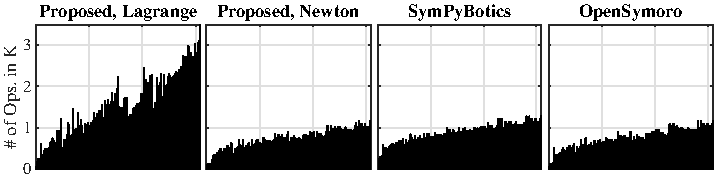
\includegraphics{statistics_serrob_numops_histogram.pdf}
	\vspace{-0.8cm}
	\caption{Comparison of the number of operations for inverse dynamics of the proposed toolbox with two methods (Lagrange, Newton-Euler) and two reference toolboxes (SymPyBotics, OpenSymoro) over all 616 serial kinematics on the horizontal axis. Sorted by increasing total number of joints and then by number of revolute joints.}
	%\vspace{-0.5cm}
	\label{fig:comparison_numops}
\end{figure} 

Code generation for parallel robots shows that the selected symbolic approach \cite{AbdellatifHei2009} of property~\ref{prop:parabdellatif} in Sec.\,\ref{sec:fundamentals_parallel} is very efficient for simple kinematic structures with a low number of kinematic parameters (resulting from a low number of mechanical joints).
For general kinematic leg chains with revolute joints instead of universal and spherical joints, the necessary computation time can reach several days and is not feasible any more.
The case of parallel robots with platform coupling joints that are not spherical is not included in the symbolic approach \cite{AbdellatifHei2009}.
In summary, only symbolic code for 91 parallel robot models was included in the database, which in total consists of a few thousand symmetric parallel robots with 3 to 6 platform degrees of freedom (DoF).
To perform dynamics simulations for parallel robots therefore the approach \cite{DoThanhKotHeiOrt2009b} of property~\ref{prop:par_dothanh} in an extended formulation is used, allowing also robots with non-spherical coupling joints.

Only some examples of industrial robots with closed loops are implemented manually, such as robot palletizers (see Fig.\,\ref{fig:robot_examples},b or Fig.\,\ref{fig:robot_examples_hybrid},a) and the 2-DoF pick-and-place machine for conveyor belts from Fig.\,\ref{fig:robot_examples_hybrid},b.
An automated systematic synthesis of serial-hybrid robots or parallel robots based on serial-hybrid leg chains as (the manually created example) in Fig.\,\ref{fig:robot_examples_hybrid},c is not implemented yet.

\begin{figure}[tb]
%\small % for caption in the figure
%\vspace{-0.6cm}
\input{../figures/robot_examples_hybrid.pdf_tex}
\vspace{-0.6cm}
\caption{Examples of hybrid robots implemented in the program framework.} %  Blue joints are passive and red joints active (with motor).
\vspace{-0.1cm}
\label{fig:robot_examples_hybrid}
\end{figure} 

\section{Conclusion}
\label{sec:conclusion}

The presented new toolchain for robot dynamics stands out against existing tools by focusing on an integral approach of a complete workflow from a robot definition to a stand-alone dynamics model implementation.
Quality requirements, such as automatic documentation and testing, are explicitly considered.
No additional steps have to be performed by the user, such as manually post-processing toolbox output or testing the results beyond integration tests.
This allows the deployment as a model generator for an extensive robot database which is used for a dimensional synthesis over all existing robots to find the best robot for a specified task.

\section*{Acknowledgements}

This work was developed over five years using funding from the German Research Foundation (DFG, grant 341489206), the Federal Ministry of Education and Research of Germany (BMBF, grant 16SV6175) and the European Union's Horizon 2020 research and innovation programme (grant 688857).

% ---- Bibliography ----
\bibliographystyle{splncs04}
\bibliography{references}
\end{document}
